%% Beispiel-Präsentation mit LaTeX Beamer im KIT-Design
%% entsprechend den Gestaltungsrichtlinien vom 1. August 2020
%%
%% Siehe https://sdqweb.ipd.kit.edu/wiki/Dokumentvorlagen

%% Beispiel-Präsentation
\documentclass{sdqbeamer} 
 
%% Titelbild
\titleimage{banner_2020_kit}

%% Gruppenlogo
\grouplogo{} 

%% Gruppenname und Breite (Standard: 50 mm)
\groupname{Department of Informatics -- Institute of Information Security and Dependability (KASTEL)}
%\groupnamewidth{50mm}

% Beginn der Präsentation

\title[Rust \& Refinement Types]{Corten: Refinement Types for Imperative Languages with Ownership}
\subtitle{Abschlusspräsentation Masterarbeit} 
\author[Carsten Csiky]{Carsten Csiky}

\date[26.\,10.\,2022]{26th Oktober 2022}

% Literatur 
 
\usepackage[citestyle=alphabetic-verb,bibstyle=numeric,hyperref,backend=biber]{biblatex}
\addbibresource{presentation.bib}
\bibhang1em

\usepackage{minted}
\usepackage{mathtools}
\usemintedstyle{colorful}
\setminted{autogobble, mathescape, highlightcolor=kit-orange60}

\usepackage{mathpartir}
\usepackage{hyperref}
\usepackage{ stmaryrd }
\usepackage{xcolor}
\usepackage[overridenote, notesposition=right]{pdfpc}
\newcommand{\code}[1]{\texttt{#1}}
\newcommand{\tuple}[2]{\langle #1 \mid #2 \rangle}
\newcommand{\set}[1]{\left\{ #1 \right\}}
\newcommand{\bbracket}[1]{\llbracket #1 \rrbracket}
\newcommand{\red}[1]{\color{kit-red90}{ #1 }}
\newcommand{\fline}[1]{\overline{\vphantom{\mid}#1}} 


\DeclareMathOperator{\rref}{ref}
\DeclareMathOperator{\dom}{dom}
\DeclareMathOperator{\img}{img}

\begin{document}
 
%Titelseite
\KITtitleframe

%Inhaltsverzeichnis
\begin{frame}{Inhaltsverzeichnis}
\tableofcontents
\end{frame}

\section{Motivation}


\begin{frame}[fragile]{Motivation}{}
  \begin{columns}
    \column{0.5\textwidth}
    \begin{minted}[autogobble]{java}
      public IntList square(IntList list) {
        return list.map(x -> x*x);
      }
    \end{minted}

    \column{.5\textwidth}
    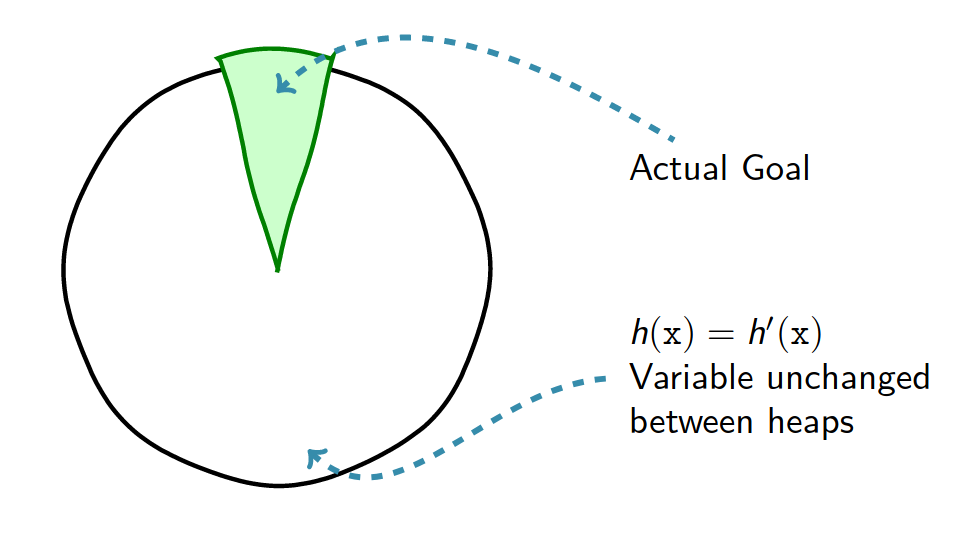
\includegraphics[width=1\textwidth]{../ratio-xkcd.png}
  \end{columns}
\end{frame}

\begin{frame}[fragile]{Motivation}{}
 \begin{minted}[autogobble]{rust}
    fn max(a: i32, b: i32) {
      if a > b { a } else { b }
    }
 \end{minted}
 \begin{itemize}
  \item<2-> $\text{Return Value }(v): v \geq a \wedge v \geq b$
  \item<3-> Rondon et al. \cite{rondon_liquid_2008}: Refinement Types for Functional Programming Languages
 \end{itemize}
 \note{
  - In BA: FP-Patterns in imperativen Programmier Sprachen.\\
  - Aufgefallen: \\
    - Eigentliches Ziel: nicht so schwer, aber\\
    - Abwesenheit von unabhängigen Änderungen verbraucht großteil der Zeit\\
  - Also: welche alternativen gibt es?\\
  - Refinement Types
 }
\end{frame}


\begin{frame}[fragile]{Motivation}{}
  \begin{minted}[autogobble]{rust}
    //@ max(a: i32, b: i32) -> {v:i32 | v >= a && v >= b }
    fn  max(a: i32, b: i32) -> i32 {
      if a > b { a } else { b }
    }
  \end{minted}
  \note{
    Wie funktioniert das?\\
    \\
    1. Extra Typ Spezifikation \\
    2. Ausdruck in klammern ähnlich zu set compresension (erlaubte werte) \\
    \\
    => Wie werden diese typen überprüft?
  }
\end{frame}


\begin{frame}[fragile]{Motivation}
  \begin{minted}[autogobble]{rust}
    //@ max(a: i32, b: i32) -> {v:i32 | v >= a && v >= b }
    fn  max(a: i32, b: i32) -> i32 {
      if a > b { a } else { b }
    }
  \end{minted}
  \begin{align*}
    &\text{let } \Gamma = (a : \{ v : \code{i32} \mid \text{true}\}, b : \{ v : \code{i32} \mid \text{true}\}) \text{ and } \tau = 
    \{ v: \code{i32} \mid v \geq a \wedge v \geq b \}
    \\
    &\inferrule*
      {
        \onslide<2->{
          \inferrule*
          { \onslide<4->{
              \inferrule*
              {\star}
              {\Gamma, a > b \vdash a : \{ v : \code{i32} \mid v \doteq a\}}
            }
            \\
              \onslide<3->{
                \inferrule*
                { 
                  \onslide<5->{
                    \text{SMT-VALID}
                    \footnotesize{
                      \left(
                      \begin{aligned}[]
                        & \, \text{true} \wedge \text{true} \wedge a > b \\
                        &\ \wedge v \doteq a \\
                        &\quad \implies (v \geq a \wedge v \geq b)
                      \end{aligned}
                      \right)
                    }
                  }
                }
                {\Gamma, a > b \vdash \{ v : \code{i32} \mid v \doteq a\} \preceq \tau}
              }
          }
          {
            \Gamma, a > b \vdash a : \tau
          }
        }
        \\
          \onslide<2->{
            \inferrule*
            {\onslide<6->{\vdots}}
            {\Gamma, \neg(a > b) \vdash b : \tau}
          }
      }
      {\Gamma \vdash \code{if } a > b\ \{ a \} \code{ else } \{ b \} : \tau}
  \end{align*}
  \note{
    0. Ziel: Prüfe Body gegen signatur \\
    1. Abkürzungen \\
    2. Funktionskörper muss return type haben; Ctx enthält die argumente (uneingeschränkt -> true predicate) \\
    3. Beide Seiten: if und else \\
      - Füge path condition zu context hinzu \\
    4. Zentrale Idee: Subtyp einführen, der bekannt ist. Hier kann etwas kreativität gebraucht werden. (Liquid Types) \\
    5. Spezifischerer Type folg trivialerweise aus Regeln \\
    6. Was bedeutet Subtyp? Predikate müssen sich implizieren (in CTX) (Liskov Substitutions Prinzip) \\
    \\
    ---- \\
    \\
    Anmerken: Zusammenarbeit von Type-System (für grobes) und SMT / Logic für kompliziertes
    \\
    Funktioniert gut, aber was ist mit mutabillity?
  }
\end{frame}



\begin{frame}[fragile]{Motivation}{}
  \begin{columns}
    \column{.5\textwidth}
    \begin{minted}[autogobble]{rust}
      fn  clamp(a: &mut i32, b: i32) {
        if *a > b { *a = b }
      }
    \end{minted}
    \begin{onlyenv}<2->
      \begin{minted}[autogobble]{rust}
        fn  client(...) {
          ...
          clamp(&mut x, 5);
          clamp(&mut y, 6);
          print!(x);
          ...
        }
      \end{minted}
    \end{onlyenv}

    \column{.5\textwidth}<3->
    What does this it \code{print(x)} output?
    \begin{itemize}
      \item In most imperative programming languages:
      \begin{itemize}
        \item Could be: old \code{x} or \code{5}
        \item<4-> But also \code{6} (if x aliases with y)!
      \end{itemize}
      \item<5-> In Rust:
        \begin{itemize}
          \item Just old \code{x} or \code{5}
          \item And nothing else!
        \end{itemize}
    \end{itemize}
    
  \end{columns}
  \note{
    - Hier: `clamp` stellt sicher, dass der referenzierte wert max `b` groß ist \\
    - Neu: `client`. Zeigt zusätzliche schwierigkeiten.\\
    -  Zwei Aufrufe an clamp. \\
    - `print` macro call to output \\
      - Welche Werte könnte `x` haben? \\
      - Auf jeden Fall mal: `x` und `5` (je nachdem was größer) \\
      - Aber! auch 6 \\
      - In Rust: Nur `x, 5'. Das liegt an ...
  }
\end{frame}



\begin{frame}[fragile]{Motivation}{}
  \begin{columns}
    \column{.5\textwidth}
    \begin{minted}[autogobble]{rust}
      fn  clamp(a: &mut i32, b: i32) { 
        // borrows a
        // owns b
        if *a > b { *a = b }
        // "returns" the borrow of a
      }
      fn  client(...) { // owns x, y
        ...
        clamp(&mut x, 5); // lend x mutably
        clamp(&mut y, 6); // lend y mutably
        print!(x);
        ...
      }
    \end{minted}

    \column{.5\textwidth}
    \begin{greenblock}{Ownership in Rust: Mutability XOR Aliasing}
      Each lexical scope tracks permissions for visible memory objects.
      Possible Permission Levels:
      \begin{itemize}
        \item Owner (e.g. \code{b})
          \begin{itemize}
            \item can: read, write
            \item transfer ownership (if no outstanding borrows)
          \end{itemize}
        \item Mutable Reference (e.g. \code{\&mut x})
          \begin{itemize}
            \item can: read, write
            \item guarantee: no aliasing
          \end{itemize}
        \item Immutable Reference (e.g. \code{\&v})
          \begin{itemize}
            \item can: read, alias
            \item guarantee: no mutation
          \end{itemize}
      \end{itemize}
    \end{greenblock}
  \end{columns}
  \note{
    - 
  }
\end{frame}


\begin{frame}[fragile]{Motivation}{}
  \begin{columns}
    \column{.5\textwidth}
      Consequences:
      \begin{itemize}
        \item unique data owner
        \item no global, mutable state
        \item no cycles in memory structure
      \end{itemize}

      \onslide<2->{
        Used for:
        \begin{itemize}
          \item safe non-gc memory management
          \item safe concurrency
          \item safe low-level hardware access
          \item \dots
          \item<3-> $\Rightarrow$ show: program verification as well
        \end{itemize}
      }
    \column{.5\textwidth}
    \begin{greenblock}{Ownership in Rust: Mutability XOR Aliasing}
      Each lexical scope tracks permissions for visible memory objects.
      Possible Permission Levels:
      \begin{itemize}
        \item Owner (e.g. \code{b})
          \begin{itemize}
            \item can: read, write
            \item transfer ownership (if no outstanding borrows)
          \end{itemize}
        \item Mutable Reference (e.g. \code{\&mut x})
          \begin{itemize}
            \item can: read, write
            \item guarantee: no aliasing
          \end{itemize}
        \item Immutable Reference (e.g. \code{\&v})
          \begin{itemize}
            \item can: read, alias
            \item guarantee: no mutation
          \end{itemize}
      \end{itemize}
    \end{greenblock}
  \end{columns}
  \note{
    - Jeder speicherobjekt hat genau einen eigentümer \\
    - Kein globaler, der veränderbar ist \\
    - Keine Zyklen in der Speicherstruktur \\
    \\ ---- \\
    - Nützlich: \\
      - wenn kein eigentümer -> speicherplatz freigeben \\
      - nur 1 mutable => keine race conditions => nützlich für concurrency \\
      - ... \\
      - In MA zeigen: auch für verifikation\\
  }
\end{frame}

\begin{frame}{Contributions}
  \begin{columns}
    \column{.5\textwidth}
    \begin{itemize}
      \item Empirical Use-Case Analysis
      \item Refinement Type System
      \begin{itemize}
        \item Automatic \& Decidable Type Checking
        \item Path Sensitivity
        \item Mutable Data \& References
        \item Modularity
        \item Partial, Mechanized Proof of Soundness
      \end{itemize}
      \item Implementation
      \begin{itemize}
        \item Accessible Interface
        \item Type-Error Messages with Source Code Locations
        \item Counter-Example Generation
      \end{itemize}
      \item Evaluation
      \begin{itemize}
        \item Automatic Verification of non-trivial Programs
        \item Comparison to other tools
      \end{itemize}
    \end{itemize}

    \column{.5\textwidth}
    \onslide<2->{
      Restrictions
      \begin{itemize}
        \item No Inference System
        \item Datatypes: Integers, Booleans and References
      \end{itemize}
    }
  \end{columns}
  \note{
    1. Wie werden mutability etc. in Rust genutzt? \\
    2. Type System entworfen. \\
      - Mit verteilhaften eigenschaften von Refinement Types \\
      - Zusätzlich: Mutable Data und Referenzen \\
      - Außerdem: Rechfertigung, Teilw. computer gestützt in Lean \\
    \\ ---- \\
    Also: Wir haben gesehen: Refinement Types gut für immutable data; Rust: eingeschränkte mutability
    => Wie zusammenbringen?
  }
\end{frame}


\section{Type System}

\begin{frame}{Overview}
  \begin{columns}
    \column{.5\textwidth}
    \begin{itemize}
      \item Common Refinement Types
      \item Mutable Values
      \item Mutable References
      \item Function Calls 
      \item Verification of \code{clamp} Example
      \item Demonstration
    \end{itemize}
    \column{.5\textwidth}

    \inputminted[fontsize=\footnotesize]{rust}{./snippets/clamp-with-spec.rs}
  \end{columns}
  \note{
    Ziel: Bsp rechts
  }
\end{frame}

\begin{frame}[fragile]{Refinement Types for Rust -- Syntax}
  \begin{columns}
    \column{.5\textwidth}
      \begin{onlyenv}<1>
        \begin{minted}[autogobble]{rust}
          fn max(a: i32, b: i32) -> i32 {
            if a > b { a } else { b }
          }
        \end{minted}
      \end{onlyenv}
      \begin{onlyenv}<2>
        \begin{minted}[autogobble]{rust}
          fn max(
            a: ty!{ av: i32 | true }, 
            b: ty!{ bv : i32 | true }
          ) -> ty!{ v : i32 | v >= av && v >= bv } {
            if a > b { a } else { b }
          }
        \end{minted}
      \end{onlyenv}
      \begin{onlyenv}<3->
        \begin{minted}[autogobble]{rust}
          fn max(
            a: ty!{ av: i32 }, 
            b: ty!{ bv : i32 }
          ) -> ty!{ v : i32 | v >= av && v >= bv } {
            if a > b { a } else { b }
          }
        \end{minted}
      \end{onlyenv}

    \column{.5\textwidth}
    \begin{itemize}
      \item Embedding using a Macro
      \item $\code{ty!}\{ l : b \mid \varphi \}$ in place of a type
      % \item \mintinline{rust}{relax_ctx!{ ... }} in place of a statement
    \end{itemize}
  \end{columns}
  \note{
    - Hinzugefügt: Macro in Rust zum verfeinern eines Typs.  \\
      - Logik Variable (anderer Scope) \\
      - Basis Typ \\
      - predikat (in Rust syntax, eingeschränkte Ausdrucksstärke) \\

  }
\end{frame}

\begin{frame}[fragile]{Type Updates}
  \begin{columns}
    \column{.5\textwidth}
    \begin{onlyenv}<1-2>
      \begin{minted}[autogobble, mathescape]{rust}
        fn incr() -> ty!{ w : i32 | w > 0 } {
         let mut i = ... as ty!{ v: i32 | v >= 0 };
         i = i + 1;
         i
        }
      \end{minted}
    \end{onlyenv}
    \only<3>{
      \inputminted[]{rust}{./snippets/decr.rs}
    }
    \only<4>{
      \inputminted[highlightlines=3]{rust}{./snippets/decr.rs}
    }
    \only<5>{
      \inputminted[highlightlines=5]{rust}{./snippets/decr.rs}
    }
    \only<6>{
      \inputminted[highlightlines=2-6]{rust}{./snippets/decr.rs}
    }

    \column{.5\textwidth}
    \only<1>{
      \begin{itemize}
        \item Types need to change through execution
        \begin{itemize}
          \item $\Rightarrow$ Type Updates
          \item $\Gamma \vdash s \Rightarrow \Gamma'$ (Statement Type Checking)
          \item $\Gamma \vdash e : \tau$ (Expression Typing)
        \end{itemize}
      \end{itemize}
    }
    \only<2-3>{
      \begin{itemize}
        \item Type of \code{i} after decrementing?
        \begin{itemize}
          \item Naïve: \code{ty!\{ v : i32 | v = v + 1 \}}
        \end{itemize}
        \item How to keep type context consistent?
        \begin{itemize}
          \item separation of program-variables and logic-variables
          \item $\Gamma$: association of program- to logic-variables and predicate
          \item on assignment: \textit{replace} association, \textit{append} predicate
          \item observation: assignments can not invalidate existing predicates
        \end{itemize}
      \end{itemize}
    }
    \only<4>{
      \begin{align*}
        &\inferrule*[left=Intro-Sub]
          {
            \Gamma \vdash e : \tau
            \\ \Gamma \vdash \tau \preceq \tau'
          }
          {\Gamma \vdash e \texttt{ as } \tau': \tau'}
        \\
        &\inferrule*[left=Decl]
          { \Gamma \vdash e :  \{ \beta : b \mid \varphi \} }
          { \Gamma \vdash \code{let } x = e  \Rightarrow \Gamma[ x \mapsto \beta], \varphi }
      \end{align*}
    }
    \only<5>{
      \begin{align*}
        &\inferrule*[left=BinOp]
          {\Gamma \vdash \alpha \text{ fresh}}
          {\Gamma \vdash x_1 \odot x_2 : \{ \alpha: b \mid \alpha \simeq \bbracket{x_1 \odot x_2}\Gamma \} }
        \\
        &\inferrule*[left=Assign]
          {\Gamma \vdash e : \{ \beta : b \mid \varphi \}}
          {\Gamma \vdash x = e \Rightarrow \Gamma[x \mapsto \beta], \varphi}
      \end{align*}
    }
    \only<6>{
      \begin{align*}
        &\inferrule*[left=Seq]
          {
            \Gamma \vdash s_1 \Rightarrow \Gamma'
            \\ \Gamma' \vdash s_2 \Rightarrow \Gamma''
          }
          {\Gamma \vdash s_1 ; s_2 \Rightarrow \Gamma''}
      \end{align*}
    }
  \end{columns}
    \note{
      - Bsp: incr i und geben den wert zurück.  \\
      - Laut signatur: Rückgabe wert negativ, aber typ: nicht-positiv, (könnte 0 sein) \\
      - Bsp. zeigt: Änderungen der Typen Notwenig. (sonst return nicht erfüllt) \\
      \\ --- \\
      Erzetze Zuordnung, Füge Predikat hinzu
    }
\end{frame}

% \begin{frame}[fragile]{Refinement Types for Rust -- Type Checking}
%   \begin{minted}[autogobble]{rust}
%     fn max(a: ty!{ av: i32 }, b: ty!{ bv : i32 }) -> ty!{ v : i32 | v >= av && v >= bv } {
%       let gt = a > b; if gt { a as ty!{ r : i32 | r >= av && r >= bv } } else { b } }
%   \end{minted}
%   \begin{align*}
%     &\text{let } \Gamma = (\set{a \mapsto av, b \mapsto bv}, \text{true} \wedge \text{true}) \text{ and } 
%       \varphi_r = (v \geq a \wedge v \geq b) \text{ and } \Gamma_1 = \Gamma[gt \mapsto v_1], v_1 \doteq av > bv
%     \\
%     &\inferrule*
%       {
%         \inferrule*
%           { 
%             \inferrule*
%               { \Gamma \vdash v_1 \text{ fresh}}
%               { \Gamma \vdash a > b : \set{v_1 : b \mid v_1 \simeq \bbracket{a > b}\Gamma } }
%           }
%           {\Gamma \vdash \code{let gt = } a > b \Rightarrow \Gamma[\code{gt} \mapsto v_1], v_1 \doteq av > bv}
%         \\ 
%           \inferrule*
%             {\Gamma_1, v_1 \doteq \text{true} \vdash a}
%             {\Gamma_1 \vdash \code{if } gt\ \{ a \} \code{ else } \{ b \} \Rightarrow \Gamma_1}
%       }
%       {\Gamma \vdash \code{let gt = } a > b; \code{if } gt\ \{ a \} \code{ else } \{ b \} \color{kit-red80}{\Rightarrow \Gamma}}
%       \\
%       &v_1 \simeq \bbracket{\code{a > b}}\Gamma = (v_1 \doteq (av > bv))
%   \end{align*}


% \end{frame}


\begin{frame}[fragile]{References -- Strong Updates}
  \begin{columns}
    \column{.55\textwidth}
    \only<1>{ \inputminted[]{rust}{./snippets/strong-updates.rs} }
    \only<2>{ \inputminted[highlightlines=2]{rust}{./snippets/strong-updates.rs} }
    \only<3>{ \inputminted[highlightlines=4]{rust}{./snippets/strong-updates.rs} }
    \only<4>{ \inputminted[highlightlines=5]{rust}{./snippets/strong-updates.rs} }
    \only<5>{ \inputminted[highlightlines=6]{rust}{./snippets/strong-updates.rs} }
    \only<6>{ \inputminted[highlightlines=8]{rust}{./snippets/strong-updates.rs} }

    \column{.45\textwidth}
    \only<2> {
      \begin{align*}
        &\inferrule*[left=Lit]
          {\Gamma \vdash \alpha \text{ fresh}}
          {\Gamma \vdash v: \{ \alpha : b \mid \alpha \simeq \bbracket{v}\Gamma\} }
      \end{align*}
    }
    \only<3> {
      \begin{align*}
        &\inferrule*[left=Ref]
          {\Gamma \vdash \alpha \text{ fresh}}
          {\Gamma \vdash \&x : \{ \alpha : \&b \mid \alpha \simeq \bbracket{\&x}\Gamma\}}
      \end{align*}
    }
    \only<4> {
      \begin{align*}
        &\inferrule*[left=Assign-Strong]
          {
            \Gamma(z) = \beta
            \\ \Gamma \vdash x \in \set{\&y} 
            \\ \Gamma \vdash \gamma \text{ fresh}
            % \\ \Gamma, \psi \vdash \alpha \text{ must reference } y
          }
          {\Gamma \vdash *x = z \Rightarrow \Gamma [y \mapsto \gamma], \gamma \doteq \beta}
        \\
        \\
        &(\text{Also }\textsc{Assign-Weak})
      \end{align*}
    }
    \only<6> {
      \begin{align*}
        &\inferrule*[left=Var]
          {\Gamma \vdash \alpha \text{ fresh}}
          {\Gamma \vdash x : \{ \alpha : b \mid \alpha \simeq \bbracket{x}\Gamma \} }
      \end{align*}
    }
  \end{columns}
  \only<1>{\note{
    Hier: Referenzen
  }}
  \only<2>{\note{
    Zuweisung mit Literal
  }}
  \only<3>{\note{
    - Introduce a Reference. Type simply equality with addr \\
    - Is das wirklich sicher? In Rust ja. Addr a ist wie eine stack slot (ändert sich auch nicht) \\
  }}
  \only<4>{\note{
    - Dereferenziert b\\
    - In TS: 
  }}
\end{frame}


\begin{frame}[fragile]{Mutable Arguments}
  \begin{minted}[autogobble, mathescape]{rust}
    fn clamp(a: &mut ty!{ a1 : i32 | true => a2 | a2 <= b1 }, b: ty!{ b1: i32 }) { 
      if *a > b { *a = b }
    }
    fn client() -> ty!{ v: () } {
      ...
      let max = 42;
      clamp(&mut x, max);
      x as ty!{ v : i32 | v < 43 };
    }
  \end{minted}
\end{frame}

\begin{frame}[fragile]{\alt<5->{Sub-Context}{Mutable Arguments}}
  \begin{columns}
    \column{.54\textwidth}
    \only<1> { \inputminted[]{rust}{./snippets/mut-arg.rs} }
    \only<2> { \inputminted[highlightlines=2]{rust}{./snippets/mut-arg.rs} }
    \only<3> { \inputminted[highlightlines=5-6]{rust}{./snippets/mut-arg.rs} }
    \only<4> { \inputminted[highlightlines=7-9]{rust}{./snippets/mut-arg.rs} }
    \only<5-8> { \inputminted[highlightlines={2,10}]{rust}{./snippets/mut-arg.rs} }
    \only<9->{
        $$
          \inferrule*[left=$\preceq$-Ctx]
            {
              \vDash \Phi \to \Phi'[\mu'(x) \triangleright \mu(x)\ \mid x \in \dom(\mu')]
              \\ \dom(\mu') \subseteq \dom(\mu)
            }
            {(\mu, \Phi) \preceq (\mu', \Phi')}
        $$
      }


    \column{.46\textwidth}
    \only<2>{
      \begin{itemize}
        \item $\code{ty!}\set{ \alpha : \text{b} \mid \varphi \Rightarrow \beta \mid \psi }$
        \item Callee requires $\varphi$ for reference destination $\alpha$
        \item Callee ensures $\psi$ for reference destination $\beta$
        \item Of course, multiple arguments possible
      \end{itemize}
    }
    \only<5->{
      \begin{itemize}
        \item still left: proof obligation from signature $a_2 \leq b_1$
        \item i.e. is $\Gamma_2$ a valid end-state?
        \item<6-> generalize notion of sub-types to context: sub-context
        \item<7-> expected state: $\Gamma_e = (\set{arg_0 \mapsto a_2, b\mapsto b_1}, a_2 \leq b_1)$
        \item<8-> show: $\Gamma_2 \preceq \Gamma_e$
      \end{itemize}
      
    }
  \end{columns}
\end{frame}


\begin{frame}[fragile]{Mutable Calls}
  \begin{columns}
    \column{.5\textwidth}
    \inputminted[]{rust}{./snippets/mut-arg-caller.rs}
    
    \column{.5\textwidth}
    \only<1->{
      \begin{itemize}
        \item append predicates from callee to context
        \item update association of logic variables
      \end{itemize}
    }
  \end{columns}
\end{frame}



\begin{frame}
  \centering
  \only<1> { 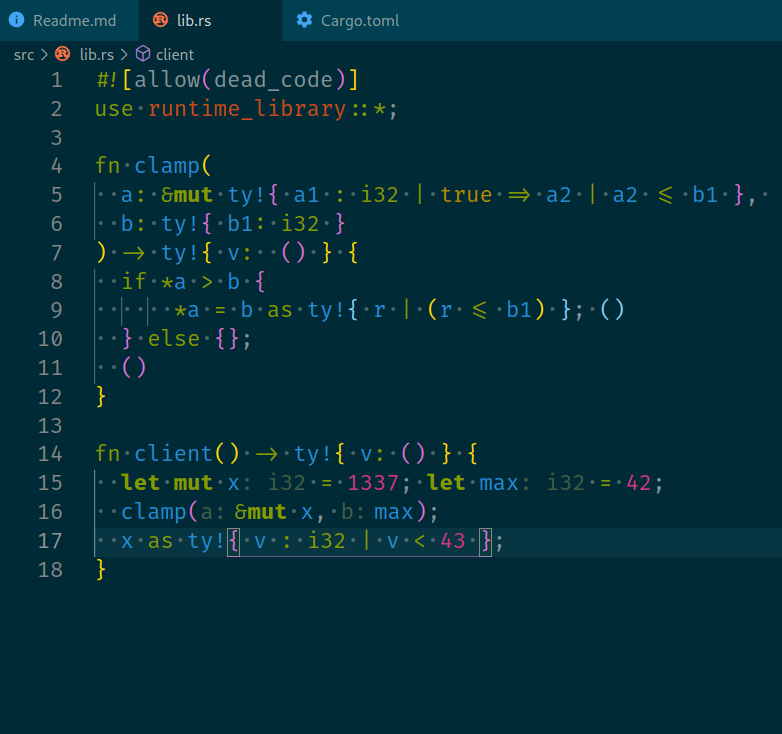
\includegraphics[width=.5\textwidth]{../demo-1.png} }
  \only<2> { 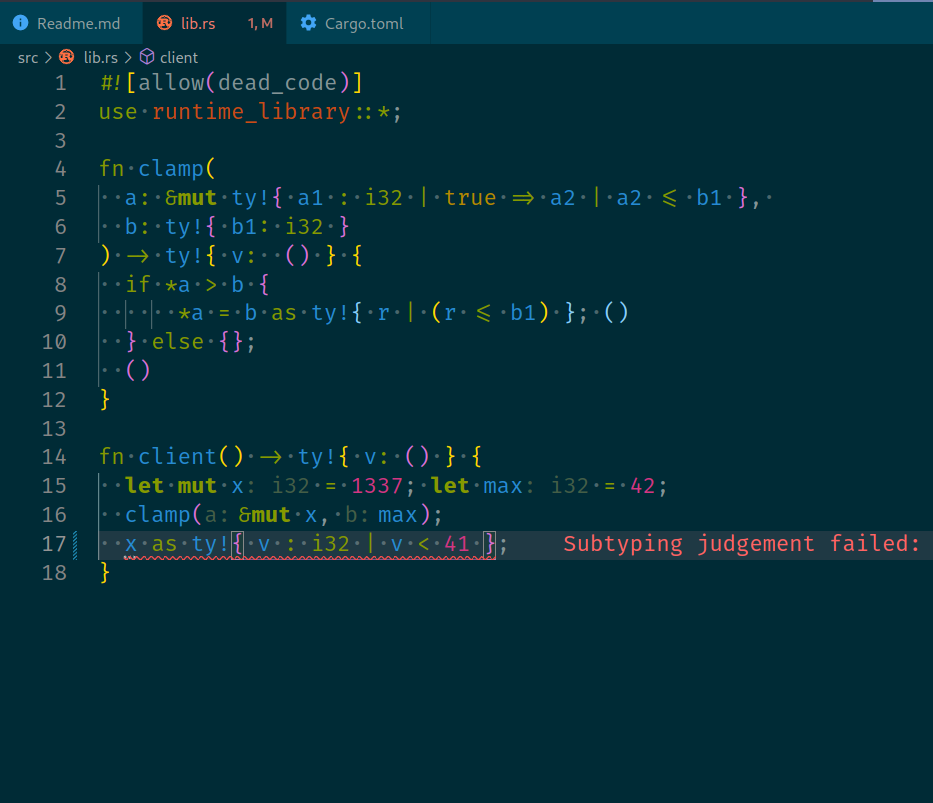
\includegraphics[width=.5\textwidth]{../demo-2.png} }
  \only<3> { 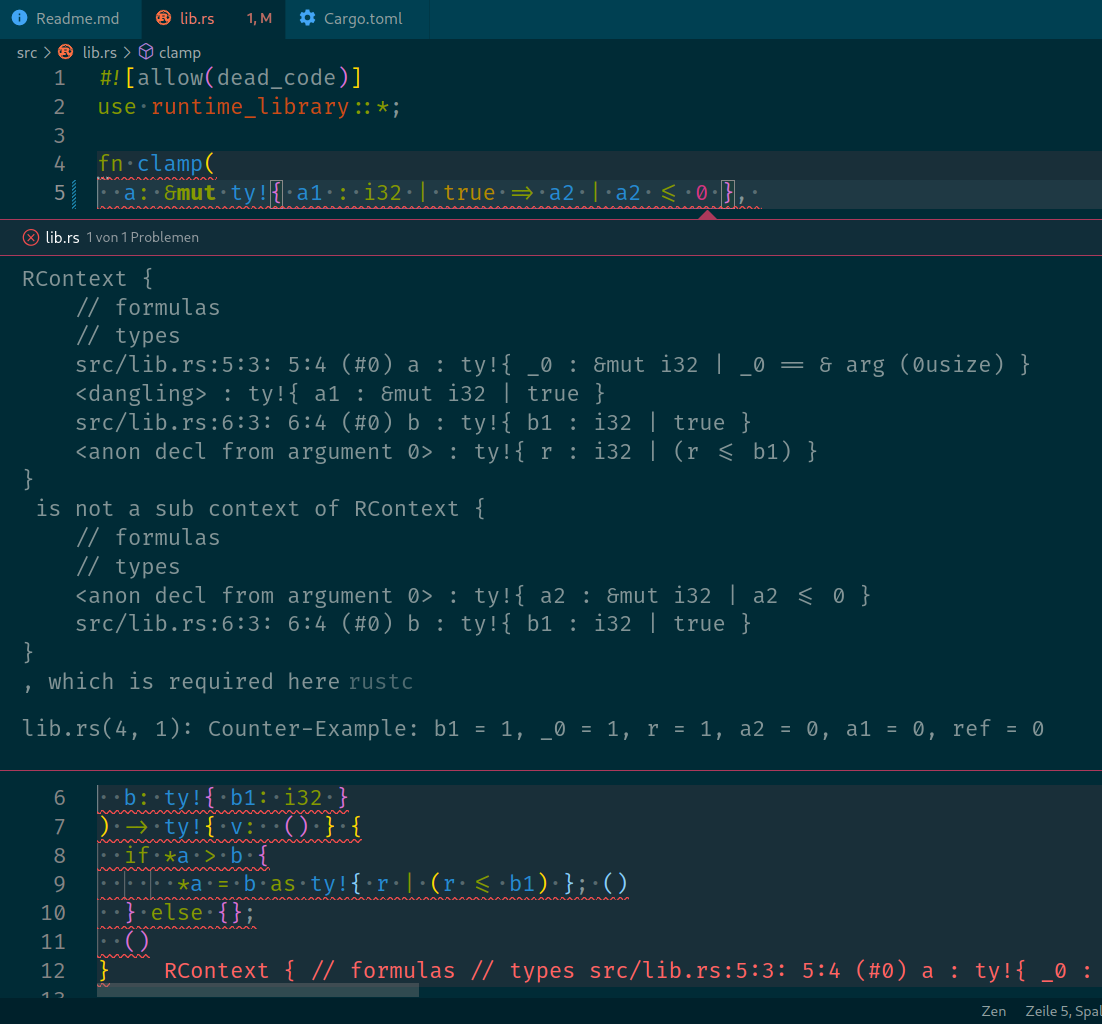
\includegraphics[width=.5\textwidth]{../demo-3.png} }
\end{frame}


\begin{frame}{SMT Request}
  \begin{columns}
    \column{.5\textwidth}
    \inputminted[mathescape=false, fontsize=\scriptsize, lastline=17]{lisp}{./snippets/smt.lisp}
    \column{.5\textwidth}

    \inputminted[mathescape=false, fontsize=\scriptsize, firstline=18]{lisp}{./snippets/smt.lisp}
  \end{columns}
  \note{
    - Ende von clamp \\
    - Genau die Sub Ctx aussage von davor \\
    \\
    1. Deklarationen \\
    2. Predikate des SubCtx \\
    3. Predikate des SuperCtx, aber negiert
  }
\end{frame}

\section{Soundness Justification}

\begin{frame}[fragile]{Soundness}
  \begin{greenblock}{Progress}
    If $\Gamma \vdash s_1$, $\sigma : \Gamma \Rightarrow \Gamma_2$ and $s_1 \neq \code{unit}$, then there is a $s_2$ and $\sigma_2$ with $\tuple{s_1}{\sigma_1} \leadsto \tuple{s_2}{\sigma_2}$.
  \end{greenblock}

  Corten strictly refines the base language, therefore progress depends on base type system.

  \begin{greenblock}{Preservation}
    If $\Gamma \vdash s \Rightarrow \Gamma_2$, $\sigma : \Gamma$ and $\tuple{s}{\sigma} \leadsto \tuple{s_1}{\sigma_1}$, then there is a $\Gamma_1$ with $\Gamma_1 \vdash s_1 \Rightarrow \Gamma_2$ and $\sigma_2 : \Gamma_2$
  \end{greenblock}

  Stronger property than base language preservation: Show that refined types are preserved\\
  
  Partial, Mechanized Proof in Lean 4
\end{frame}

\begin{frame}[fragile]{State Conformance}
  \begin{greenblock}{State Conformance $\sigma : \Gamma$}
    A state $\sigma$ is conformant with respect to a typing context $\Gamma = (\mu, \Phi)$ (written as $\sigma : \Gamma$), iff:
    $$
      \Phi[\mu(x) \triangleright \bbracket{\sigma(x)} \mid x \in \dom(\mu)] \text{ is satisfiable}
    $$
    I.e. a conformant type context does not contradict the execution state.
  \end{greenblock}
  Examples:
  \begin{itemize}
    \item If $\sigma : (\emptyset, \Phi)$ then $\Phi$ is satisfiable
    \item If $\sigma : (\mu, \Phi_1 \wedge \Phi_2)$ then $\sigma : (\mu, \Phi_1)$ and $\sigma : (\mu, \Phi_1)$.
    \item If $\sigma : (\mu, \Phi)$ and $\text{FV}(\Phi) \subseteq \dom(\mu)$, then $\vDash \Phi[\mu(x) \triangleright \bbracket{\sigma(x)} \mid x \in \dom(\mu)]$
  \end{itemize}
  \note{
    - Konformanz: Schon gesehen. Jetzt definierten \\
    - Ungewöhnlich, weil Kontext freie variablen enthalten kann (deswegen Erfüllbarkeit) \\
    - Beispiele: \\
      1. trivialer Fall (kein state) \\
      2. relativ offensichtlich \\
      3. interessant: Wenn keine unassociated logik variablen, dann auch allgemeingültig. (weil konstant) \\
  }
\end{frame}


\begin{frame}[fragile]{Intermediate Steps}
  \begin{greenblock}{Conformance of Symbolic Execution}
    If $\sigma : \Gamma$, $\Gamma \vdash \alpha \text{ fresh}$ then $\sigma[x \mapsto \bbracket{e} \sigma] : \Gamma[x \mapsto \alpha],(\alpha \simeq \bbracket{e} \Gamma)$
  \end{greenblock}
  where $(\alpha \simeq \bbracket{e} \Gamma)$ is the symbolic execution of $e$ equated with $\alpha$ in context $\Gamma$
  
  \begin{greenblock}{Reference Predicates are Conservative}
    If $\sigma : \Gamma $ and $\Gamma \vdash *x \in \set{y_1, \dots, y_n}$ then $\bbracket{\sigma(x)} = \&y_i$ for some $i \in 1, \dots, n$ 
  \end{greenblock}

  Rare case where conservative typing requires 

  \begin{greenblock}{Sub-Context Relation is Conservative}
    If $\Gamma \preceq \Gamma'$ and $\sigma : \Gamma$ then $\sigma : \Gamma'$
  \end{greenblock}

  \note{
    - Regel wird für zuweisung gebraucht: (`e` an `x`)
    - Gleichsetzen ist vielleicht nicht möglich (v.a. wenn logik nicht stark genug)
    ---
    - Im gegensatz zum rest: Ctx muss richtigen wert enthalten.
      - möglich wg. sehr eingeschränkter prädikate für references
    ---
    - Abschächen d. Ctx kann keine widersprüche erzeugen
    - für Fn-Call und relax ctx
  }
\end{frame}

\section{Related Work}

\begin{frame}{Related Work}
  \textbf{Refinement Types and Mutability}
  \begin{itemize}
    \item Rondon et al. \cite{rondon_low-level_2010}, Bakst and Jhala \cite{bakst_predicate_2016}: Refinement Types for C subset. Lack of guarantees requires ad-hoc mechanisms to control aliasing
    \item Lanzinger \cite{lanzinger_property_2021}: Property Types in Java (only immutable). Bachmeier \cite{bachmeier_property_2022}: Extension using Ownership System
    \item Toman et al. \cite{toman_consort_2020} (ConSORT): Fractional Ownership, strong and weak updates
  \end{itemize}
  \textbf{Rust verification}
  \begin{itemize}
    \item Ullrich \cite{ullrich_simple_2016}: Translation to Lean; linear mutation chain. Denis et al \cite{denis_creusot_2021} similar, but to Why3
    \item Astrauskas et al. \cite{astrauskas_leveraging_2019} (Prusti): heavy-weight verification, translation to separation logic (Viper)
    \item Matsushita et al. \cite{matsushita_rusthorn_2020} (RustHorn): constrained Horn clauses 
  \end{itemize}
\end{frame}

\begin{frame}{Related Work: Flux -- Refinement Types for Rust}
  \begin{columns}
    \column{.5\textwidth}
    \begin{itemize}
      \item MIR vs. HIR
      \item specification in comments vs. embedding in types
      \item context inclusions vs. sub context
      \item distinction strong and weak references vs. dynamic choice by typ checking rules
      \item explicit introduction of logic variables vs. ad-hoc
      \item formalization based on RustBelt vs. formalization based on own language
      \item missing in Corten: records \& inference
      \item otherwise: similar capabilities
    \end{itemize}

    \column{.5\textwidth}
    \inputminted[]{rust}{./snippets/flux-comparison-1.rs}
    
    \inputminted[]{rust}{./snippets/flux-comparison-2.rs}
    
  \end{columns}
  \note{
    - Paper von Authoren von Liquid Types Papern\\
    - Veröffentlicht gegen ende der MA\\
    - Pluralität: erst nach eigener arbeit untersucht
  }
\end{frame}


\section{Conclusion / Future Work}


\begin{frame}{Future Work}
  \begin{itemize}
    \item Records \& ADTs 
    \begin{itemize}
      \item More Syntax, Nested Structures
      \item Variant Distinction
    \end{itemize}
    \item Predicate Generics (Abstract Predicates)
      \begin{itemize}
        \item Uninterpreted Functions in Types
        \item Syntactic Embedding?
      \end{itemize}
    \item Concurrency using Predicate Generics?
      \begin{itemize}
        \item Use Predicate Generics
        \item Predicate describes Contract for Mutation
        \item Interesting, because unusual guarantees in Rust
      \end{itemize}
  \end{itemize}
  \note{
    - use this for concurrency. Should be interesting in Rust (b/c of guarantees)
  }
\end{frame}

\begin{frame}{Conclusion}
  \begin{columns}
    \column{.5\textwidth}
    \begin{itemize}
      \item Refinement Type System for Rust with Mutability
      \begin{itemize}
        \item Decidable, Automatic
        \item Complex Mutation Patterns
        \item ...
      \end{itemize}
      \item Minimal Interface
      \item Soundness Justification
      \item Practical Usability
      \begin{itemize}
        \item Source Locations
        \item Counter Example
        \item IDE Integration
      \end{itemize}
    \end{itemize}

    \column{.5\textwidth}
    \only<2->{
      More Information:
      \begin{itemize}
        \item Implementation, Thesis, Mechanized Proof, Evaluation: \url{https://gitlab.com/csicar/liquidrust}
        \item Empirical Analysis: \url{https://gitlab.com/csicar/crates-analysis}
      \end{itemize}
    }
  \end{columns}
\end{frame}

\begin{frame}

\end{frame}


\appendix

\beginbackup


\begin{frame}[allowframebreaks]{Literatur}
  \tiny{
    \printbibliography
  }
\end{frame}



\section{Empirical Analysis}

\begin{frame}{Empirical Use-Case Analysis}
  \begin{columns}
    \column{.5\textwidth}
    \begin{itemize}
      \item public open-source code (\text{crates.io})
      \item about 64 million lines of Rust code
      \item syntactical analysis
    \end{itemize}
    \column{0.5\textwidth}
    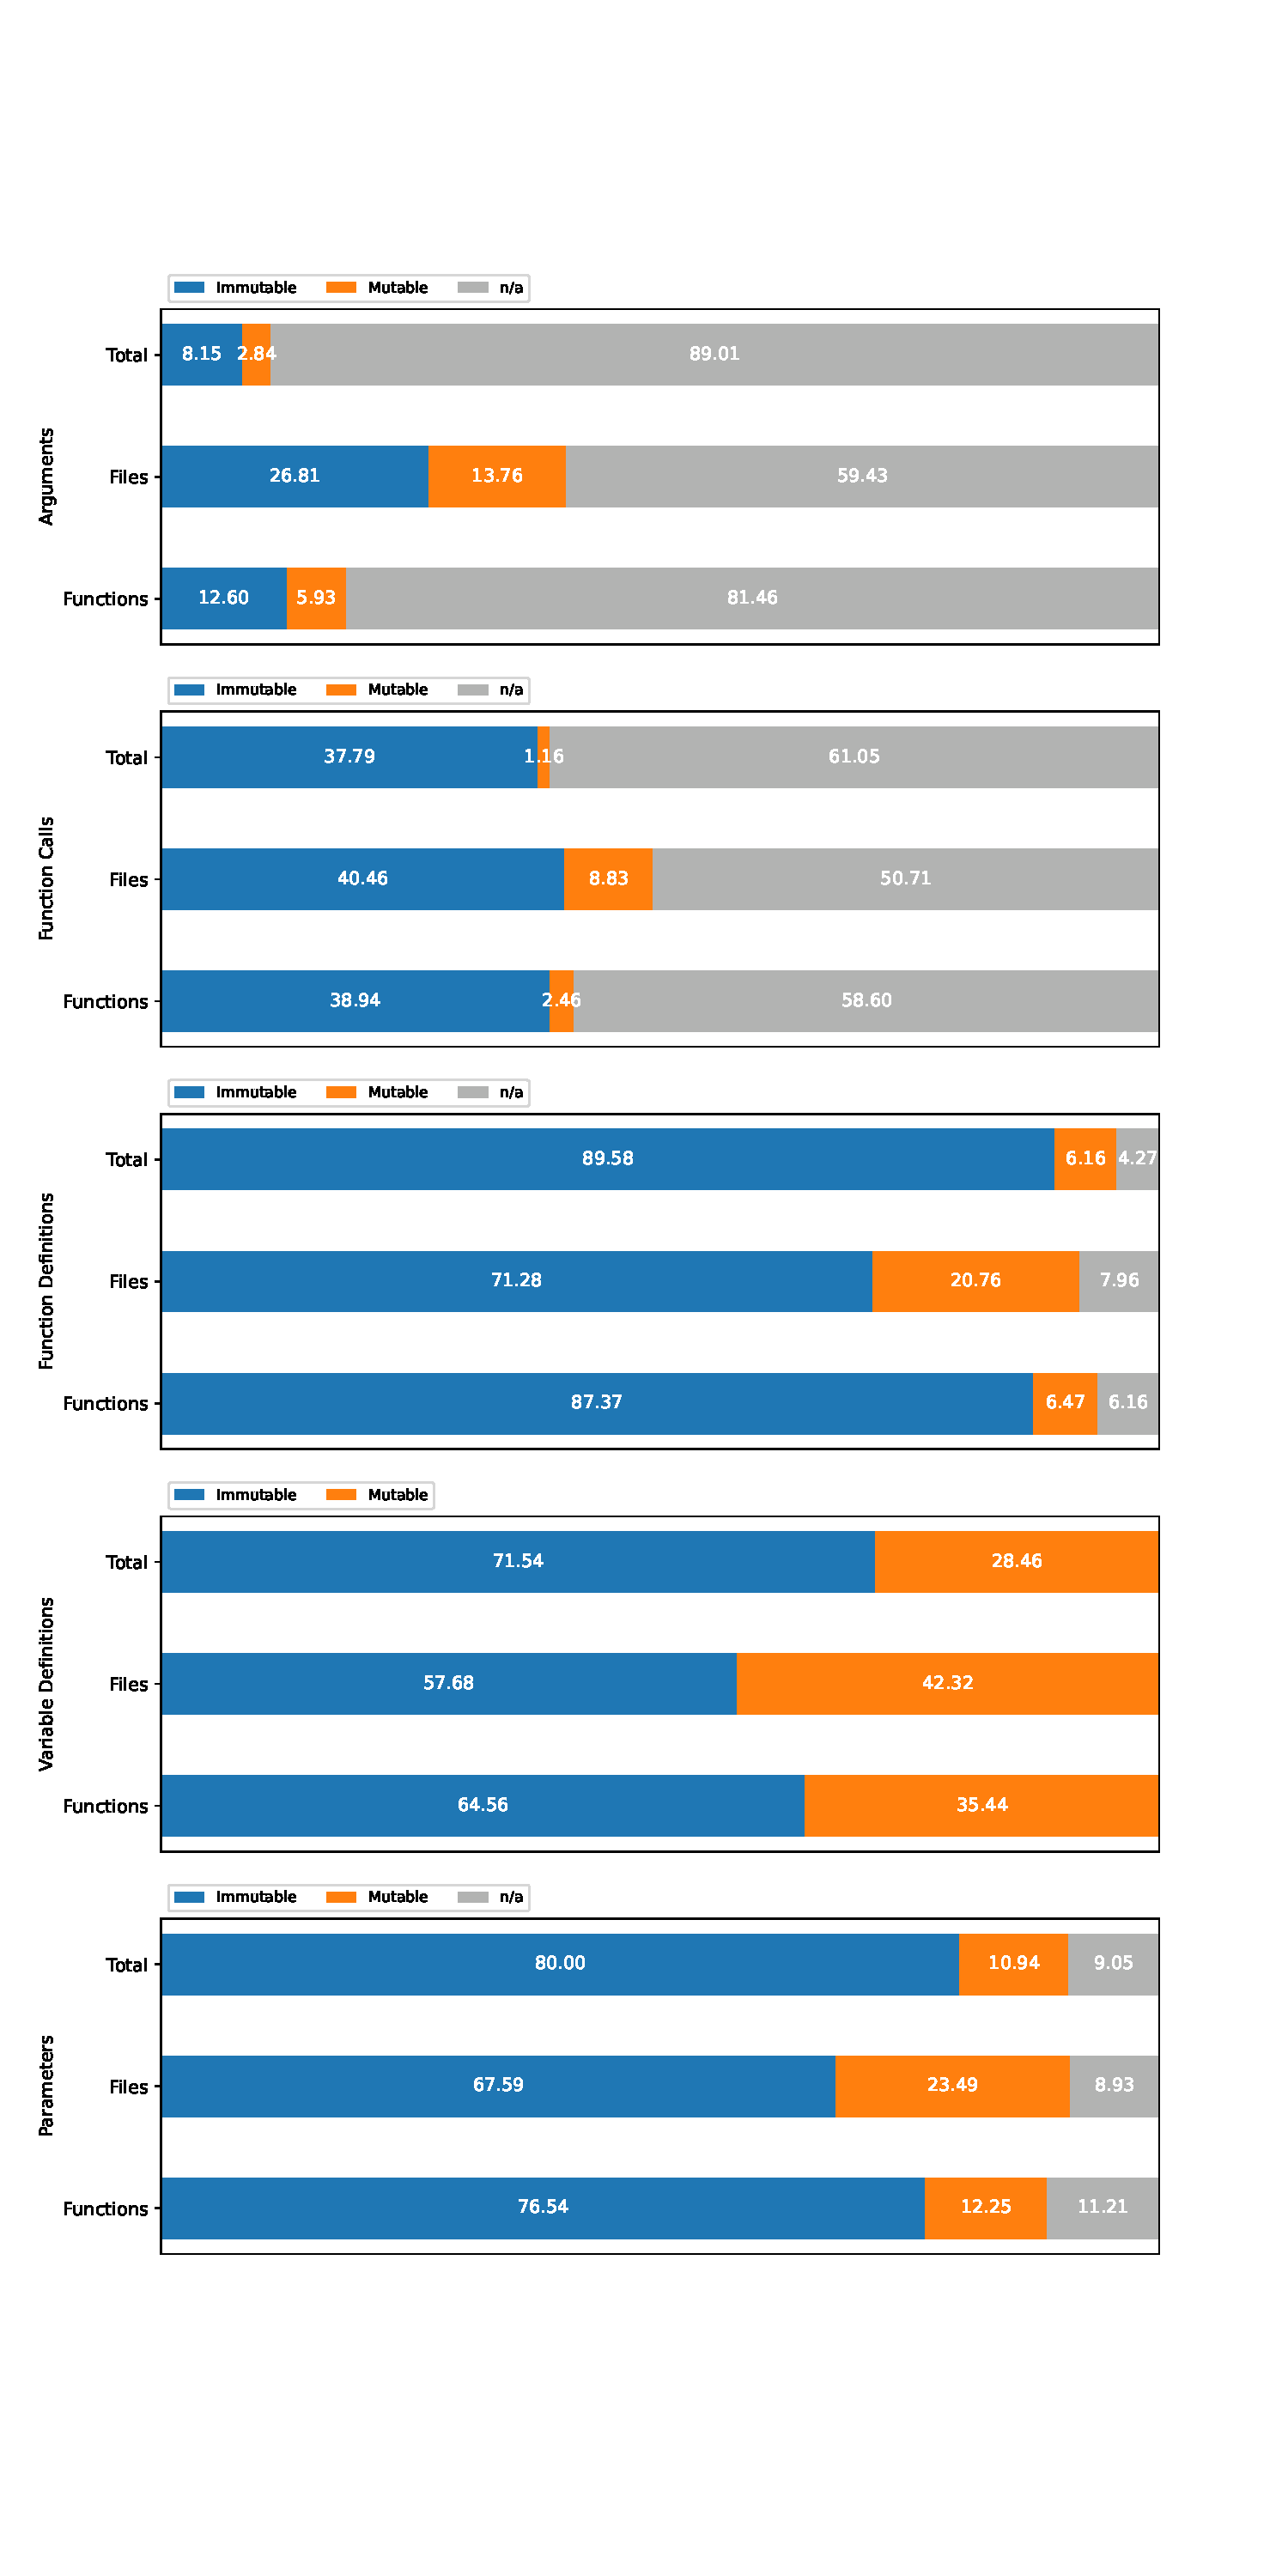
\includegraphics[width=\textwidth]{../mutability_by_category.pdf}
  \end{columns}
\end{frame}

\begin{frame}{\code{decr} Typing Tree}
  \begin{align*}
    &\text{let }
    \Gamma_2 = \Gamma[i \mapsto v_1], v > 0 \text{ and }
    \tau = \set{v : \code{i32} \mid v > 0}\\
    &\inferrule*[left=\footnotesize{Seq}]
      {
        \inferrule*[left=\footnotesize{Decl}]
          {
            \inferrule*[left=\footnotesize{Intro}-Sub]
              {\Gamma_1 \vdash ... : \tau' \\ \Gamma_1 \vdash \tau' \preceq \tau}
              {\Gamma_1 \vdash \code{... as $\tau$} : \tau}
          }
          {\Gamma_1 \vdash \code{let i = ... as $\tau$} \Rightarrow \Gamma_2}
        \\ 
        \inferrule*[left=\footnotesize{Ass}]
          {
            \inferrule*[left=\footnotesize{BinOp}]
              {\Gamma_1 \vdash v_2 \text{ fresh}}
              {\Gamma_1 \vdash \code{i - 1} : \set{v_2 : \text{i32} \mid v_2 \doteq v - 1}}
          }
          {\Gamma_2 \vdash \code{i = i - 1} \Rightarrow \Gamma[i \mapsto v_2], v > 0, v_2 \doteq v - 1}
      }
      {\Gamma_1 \vdash \code{let i = ... as $\tau$; i = i - 1} \Rightarrow \Gamma[i \mapsto v_2], v > 0, v_2 \doteq v - 1}
  \end{align*}
\end{frame}


\begin{frame}
  Expression Typing $\Gamma \vdash e : \tau$
  $$ \begin{gathered}
    \inferrule*[left=Lit]
      {\Gamma \vdash \alpha \text{ fresh}}
      {\Gamma \vdash v: \{ \alpha : b \mid \alpha \simeq \bbracket{v}\Gamma\} }
    %
    \quad
    \inferrule*[left=BinOp]
      {
        \Gamma \vdash \alpha \text{ fresh}
      }
      {\Gamma \vdash x_1 \odot x_2 : \{ \alpha: b \mid \alpha \simeq \bbracket{x_1 \odot x_2}\Gamma \} }
    %
    \\
    \inferrule*[left=Var]
      {\Gamma \vdash \alpha \text{ fresh}}
      {\Gamma \vdash x : \{ \alpha : b \mid \alpha \simeq \bbracket{x}\Gamma \} }
    %
    \quad
    \inferrule*[left=Intro-Sub]
      {
        \Gamma \vdash e : \tau
        \\ \Gamma \vdash \tau \preceq \tau'
      }
      {\Gamma \vdash e \texttt{ as } \tau': \tau'}
  \end{gathered} $$

  Statement Type Checking $\Gamma \vdash s \Rightarrow \Gamma'$

  $$ \begin{gathered}
    \inferrule*[left=If]
      {
        \Gamma, \Gamma(x) \doteq \code{true} \vdash s_t \Rightarrow \Gamma'
        \\ \Gamma, \Gamma(x) \doteq \code{false} \vdash s_e \Rightarrow \Gamma'
      }
      {\Gamma \vdash \text{if } x \text{ then }s_t\text{ else } s_e \Rightarrow \Gamma'}
    %
    \\
    \inferrule*[left=Seq]
      {
        \Gamma \vdash s_1 \Rightarrow \Gamma'
        \\ \Gamma' \vdash s_2 \Rightarrow \Gamma''
      }
      {\Gamma \vdash s_1 ; s_2 \Rightarrow \Gamma''}
    %
    \\
    \inferrule*[left=Decl]
      {
        \Gamma \vdash e :  \{ \beta : b \mid \varphi \}
      }
      {\Gamma \vdash \code{let } x = e  \Rightarrow \Gamma[ x \mapsto \beta], \varphi}
    %
    \quad
    \inferrule*[left=Assign]
      {\Gamma \vdash e : \{ \beta : b \mid \varphi \}}
      {\Gamma \vdash x = e \Rightarrow \Gamma[x \mapsto \beta], \varphi}
  \end{gathered} $$
\end{frame}


\begin{frame}[fragile]
  Expression Typing $\Gamma \vdash e : \tau$
  \begin{align*}
    \inferrule*[left=Ref]
    {\Gamma \vdash \alpha \text{ fresh}}
    {\Gamma \vdash \&x : \{ \alpha : \&b \mid \alpha \simeq \bbracket{\&x}\Gamma\}}
    %
    \\
    \inferrule*[left=Var-Deref]
      {\Gamma \vdash x \in \set{\&y} \\ \Gamma \vdash y : \tau }
      {\Gamma \vdash *x : \tau }
    \quad
  \end{align*}
  Statement Type Checking $\Gamma \vdash s \Rightarrow \Gamma'$
  \begin{align*}
    \inferrule*[left=Assign-Strong]
    {
      \Gamma(z) = \beta
      \\ {\red \Gamma \vdash x \in \set{\&y} }
      \\ \Gamma \vdash \gamma \text{ fresh}
    }
    {\Gamma \vdash *x = z \Rightarrow \Gamma [y \mapsto \gamma], \gamma \doteq \beta}
    %
    \\
    \onslide<2->{
      \inferrule*[left=Assign-Weak]
      {
        \Gamma \vdash e : \tau 
        \\ \Gamma \vdash x \in \set{\&y_1, \dots, \&y_n}
        \\\\ \fline{ \Gamma \vdash y_i : \{ \beta_i : b_i \mid \varphi_i \} }
        \\ \fline{ \Gamma \vdash \tau \preceq \{ \beta_i : b_i \mid \varphi_i \} }
      }
      {\Gamma \vdash *x = e \Rightarrow \Gamma}
    }
  \end{align*}
\end{frame}

\begin{frame}{Predicate Generics \& Concurrecy}
  \inputminted[fontsize=\footnotesize]{rust}{./snippets/concurrency.rs}
\end{frame}


\subsection{Erster Unterabschnitt}
\begin{frame}{Blöcke}{in den KIT-Farben}
  \begin{columns}
    \column{.3\textwidth}
    \begin{greenblock}{Greenblock}
      Standard (\texttt{block})
        \end{greenblock}
    \column{.3\textwidth}
    \begin{blueblock}{Blueblock}
      = \texttt{exampleblock}
        \end{blueblock}
    \column{.3\textwidth}
    \begin{redblock}{Redblock}
      = \texttt{alertblock}
        \end{redblock}
  \end{columns}
  \begin{columns}
    \column{.3\textwidth}
        \begin{brownblock}{Brownblock}
        \end{brownblock}
    \column{.3\textwidth}
        \begin{purpleblock}{Purpleblock}
        \end{purpleblock}
    \column{.3\textwidth}
        \begin{cyanblock}{Cyanblock}
        \end{cyanblock}
  \end{columns}
  \begin{columns}
    \column{.3\textwidth}
        \begin{yellowblock}{Yellowblock}
        \end{yellowblock}
    \column{.3\textwidth}
        \begin{lightgreenblock}{Lightgreenblock}
        \end{lightgreenblock}
    \column{.3\textwidth}
        \begin{orangeblock}{Orangeblock}
        \end{orangeblock}
  \end{columns}
  \begin{columns}
    \column{.3\textwidth}
        \begin{grayblock}{Grayblock}
        \end{grayblock}
    \column{.3\textwidth}
    \begin{contentblock}{Contentblock}
      (farblos)
    \end{contentblock}
    \column{.3\textwidth}
  \end{columns}
\end{frame}
    
\subsection{Zweiter Unterabschnitt}
\begin{frame}{Auflistungen}
  Text
  \begin{itemize}
    \item Auflistung\\ Umbruch
    \item Auflistung
    \begin{itemize}
      \item Auflistung
      \item Auflistung
    \end{itemize}
  \end{itemize}
\end{frame}

\section{Zweiter Abschnitt}

\begin{frame}
        Bei Frames ohne Titel wird die Kopfzeile nicht angezeigt, und  
    der freie Platz kann für Inhalte genutzt werden.
\end{frame}

\begin{frame}[plain]
    Bei Frames mit Option \texttt{[plain]} werden weder Kopf- noch Fußzeile angezeigt.
\end{frame}

\begin{frame}[t]{Beispielinhalt}
    Bei Frames mit Option \texttt{[t]} werden die Inhalte nicht vertikal zentriert, sondern an der Oberkante begonnen.
\end{frame}


\begin{frame}{Beispielinhalt: Literatur}
\end{frame}

\section{Farben}
%% ----------------------------------------
%% | Test-Folie mit definierten Farben |
%% ----------------------------------------
\begin{frame}{Farbpalette}
\tiny

% GREEN
  \colorbox{kit-green100}{kit-green100}
  \colorbox{kit-green90}{kit-green90}
  \colorbox{kit-green80}{kit-green80}
  \colorbox{kit-green70}{kit-green70}
  \colorbox{kit-green60}{kit-green60}
  \colorbox{kit-green50}{kit-green50}
  \colorbox{kit-green40}{kit-green40}
  \colorbox{kit-green30}{kit-green30}
  \colorbox{kit-green25}{kit-green25}
  \colorbox{kit-green20}{kit-green20}
  \colorbox{kit-green15}{kit-green15}
  \colorbox{kit-green10}{kit-green10}
  \colorbox{kit-green5}{kit-green5}

% BLUE
  \colorbox{kit-blue100}{kit-blue100}
  \colorbox{kit-blue90}{kit-blue90}
  \colorbox{kit-blue80}{kit-blue80}
  \colorbox{kit-blue70}{kit-blue70}
  \colorbox{kit-blue60}{kit-blue60}
  \colorbox{kit-blue50}{kit-blue50}
  \colorbox{kit-blue40}{kit-blue40}
  \colorbox{kit-blue30}{kit-blue30}
  \colorbox{kit-blue25}{kit-blue25}
  \colorbox{kit-blue20}{kit-blue20}
  \colorbox{kit-blue15}{kit-blue15}
  \colorbox{kit-blue10}{kit-blue10}
  \colorbox{kit-blue5}{kit-blue5}

% RED
  \colorbox{kit-red100}{kit-red100}
  \colorbox{kit-red90}{kit-red90}
  \colorbox{kit-red80}{kit-red80}
  \colorbox{kit-red70}{kit-red70}
  \colorbox{kit-red60}{kit-red60}
  \colorbox{kit-red50}{kit-red50}
  \colorbox{kit-red40}{kit-red40}
  \colorbox{kit-red30}{kit-red30}
  \colorbox{kit-red25}{kit-red25}
  \colorbox{kit-red20}{kit-red20}
  \colorbox{kit-red15}{kit-red15}
  \colorbox{kit-red10}{kit-red10}
  \colorbox{kit-red5}{kit-red5}

% GREY
  \colorbox{kit-gray100}{\color{white}kit-gray100}
  \colorbox{kit-gray90}{\color{white}kit-gray90}
  \colorbox{kit-gray80}{\color{white}kit-gray80}
  \colorbox{kit-gray70}{\color{white}kit-gray70}
  \colorbox{kit-gray60}{\color{white}kit-gray60}
  \colorbox{kit-gray50}{\color{white}kit-gray50}
  \colorbox{kit-gray40}{kit-gray40}
  \colorbox{kit-gray30}{kit-gray30}
  \colorbox{kit-gray25}{kit-gray25}
  \colorbox{kit-gray20}{kit-gray20}
  \colorbox{kit-gray15}{kit-gray15}
  \colorbox{kit-gray10}{kit-gray10}
  \colorbox{kit-gray5}{kit-gray5}

% Orange
  \colorbox{kit-orange100}{kit-orange100}
  \colorbox{kit-orange90}{kit-orange90}
  \colorbox{kit-orange80}{kit-orange80}
  \colorbox{kit-orange70}{kit-orange70}
  \colorbox{kit-orange60}{kit-orange60}
  \colorbox{kit-orange50}{kit-orange50}
  \colorbox{kit-orange40}{kit-orange40}
  \colorbox{kit-orange30}{kit-orange30}
  \colorbox{kit-orange25}{kit-orange25}
  \colorbox{kit-orange20}{kit-orange20}
  \colorbox{kit-orange15}{kit-orange15}
  \colorbox{kit-orange10}{kit-orange10}
  \colorbox{kit-orange5}{kit-orange5}

% lightgreen
  \colorbox{kit-lightgreen100}{kit-lightgreen100}
  \colorbox{kit-lightgreen90}{kit-lightgreen90}
  \colorbox{kit-lightgreen80}{kit-lightgreen80}
  \colorbox{kit-lightgreen70}{kit-lightgreen70}
  \colorbox{kit-lightgreen60}{kit-lightgreen60}
  \colorbox{kit-lightgreen50}{kit-lightgreen50}
  \colorbox{kit-lightgreen40}{kit-lightgreen40}
  \colorbox{kit-lightgreen30}{kit-lightgreen30}
  \colorbox{kit-lightgreen25}{kit-lightgreen25}
  \colorbox{kit-lightgreen20}{kit-lightgreen20}
  \colorbox{kit-lightgreen15}{kit-lightgreen15}
  \colorbox{kit-lightgreen10}{kit-lightgreen10}
  \colorbox{kit-lightgreen5}{kit-lightgreen5}

% Brown
  \colorbox{kit-brown100}{kit-brown100}
  \colorbox{kit-brown90}{kit-brown90}
  \colorbox{kit-brown80}{kit-brown80}
  \colorbox{kit-brown70}{kit-brown70}
  \colorbox{kit-brown60}{kit-brown60}
  \colorbox{kit-brown50}{kit-brown50}
  \colorbox{kit-brown40}{kit-brown40}
  \colorbox{kit-brown30}{kit-brown30}
  \colorbox{kit-brown25}{kit-brown25}
  \colorbox{kit-brown20}{kit-brown20}
  \colorbox{kit-brown15}{kit-brown15}
  \colorbox{kit-brown10}{kit-brown10}
  \colorbox{kit-brown5}{kit-brown5}

% Purple
  \colorbox{kit-purple100}{kit-purple100}
  \colorbox{kit-purple90}{kit-purple90}
  \colorbox{kit-purple80}{kit-purple80}
  \colorbox{kit-purple70}{kit-purple70}
  \colorbox{kit-purple60}{kit-purple60}
  \colorbox{kit-purple50}{kit-purple50}
  \colorbox{kit-purple40}{kit-purple40}
  \colorbox{kit-purple30}{kit-purple30}
  \colorbox{kit-purple25}{kit-purple25}
  \colorbox{kit-purple20}{kit-purple20}
  \colorbox{kit-purple15}{kit-purple15}
  \colorbox{kit-purple10}{kit-purple10}
  \colorbox{kit-purple5}{kit-purple5}

% Cyan
  \colorbox{kit-cyan100}{kit-cyan100}
  \colorbox{kit-cyan90}{kit-cyan90}
  \colorbox{kit-cyan80}{kit-cyan80}
  \colorbox{kit-cyan70}{kit-cyan70}
  \colorbox{kit-cyan60}{kit-cyan60}
  \colorbox{kit-cyan50}{kit-cyan50}
  \colorbox{kit-cyan40}{kit-cyan40}
  \colorbox{kit-cyan30}{kit-cyan30}
  \colorbox{kit-cyan25}{kit-cyan25}
  \colorbox{kit-cyan20}{kit-cyan20}
  \colorbox{kit-cyan15}{kit-cyan15}
  \colorbox{kit-cyan10}{kit-cyan10}
  \colorbox{kit-cyan5}{kit-cyan5}
    
\end{frame}
%% ----------------------------------------
%% | /Test-Folie mit definierten Farben |
%% ----------------------------------------
\backupend

\end{document}